%
% File acl2014.tex
%
% Contact: koller@ling.uni-potsdam.de, yusuke@nii.ac.jp
%%
%% Based on the style files for ACL-2013, which were, in turn,
%% Based on the style files for ACL-2012, which were, in turn,
%% based on the style files for ACL-2011, which were, in turn, 
%% based on the style files for ACL-2010, which were, in turn, 
%% based on the style files for ACL-IJCNLP-2009, which were, in turn,
%% based on the style files for EACL-2009 and IJCNLP-2008...

%% Based on the style files for EACL 2006 by 
%%e.agirre@ehu.es or Sergi.Balari@uab.es
%% and that of ACL 08 by Joakim Nivre and Noah Smith

\documentclass[11pt]{article}
\usepackage{acl2014}
\usepackage{times}
\usepackage{url}
\usepackage{latexsym}
\usepackage{tabulary}
\usepackage{tabulary}
\usepackage{comment}
\usepackage{graphicx}
\usepackage{array}
\usepackage{multirow}

%\setlength\titlebox{5cm}

% You can expand the titlebox if you need extra space
% to show all the authors. Please do not make the titlebox
 % smaller than 5cm (the original size); we will check this
% in the camera-ready version and ask you to change it back.

\title{Toward Macro-Insights  for Suicide Prevention: \\ Anaylzing Fine-Grain Distress at Scale}

%\author{Ravdeep Johar\\
 % Department of Computer Science \\
 % Rochester Institute of Technology \\
 % {\tt rsj7209@rit.edu} \And
 %Christopher M. Homan\\
 % Department of Computer Science \\
 % Rochester Institute of Technology \\
  %{\tt cmh@cs.rit.edu}\\\\ 
 %}

\date{March 21, 2014}

\begin{document}
\maketitle
\begin{abstract}

This paper is an initial exploratory research 
 \end{abstract}

\section{Introduction}


Suicide is among the leading causes of death for individuals 10--44 years of age in the United States \cite{heron2009deaths}. Indeed, while mortality rates for most illnesses decreased between 2008 and 2009, the rate of suicide increased by 2.4\%  \cite{heron2009deaths}. The lifetime prevalence for suicidal ideation is between 5.6 and 14.3 percent in the general population, and as high as 19.8--24.0\% among youth~\cite{nock2008suicide}. 

The first step toward suicide \emph{prevention} is to identify, ideally in consultation with clinical experts, the risk factors associated with suicide.  Due to social stigma among other sociocultural factors~\cite{crosby2011self}, individuals with suicidal ideation may not always reach out to professionals or, if they do, provide them with accurate information. They may not even realize their own level of suicide risk before it is too late. Self-reporting, then, is not a reliable means of detecting and assessing suicide risk.

 Individuals may be more inclined to seek support from informal resources, such as social media, instead of seeking treatment (Crosby et al., 2011; Bruffaerts et al., 2011; Ryan et al., 2010). Evidence suggests that youth and emerging adults usually prefer to seek help from their friends and families; however, higher levels of suicidal ideation are associated with lower levels of help-seeking from both formal or informal resources (Deane et al., 2001).  

These trends in help-seeking behavior suggests that social media might be a rich outlet for learning about support seeking.
Internet- and telecommunications-driven activity is revolutionizing the social sciences by providing data---much of it publicly available---on human activity in situ, at volumes and a level of time and space granularity never before approached. Can such data improve clinical preventative measures by providing access to at-risk individuals who would otherwise go undetected, and by leading to better science about suicide risk behaviors? 

\newcite{mann1999toward} developed the stress diathesis model for suicidal behavior, using many of the aforementioned risk factors.  This model suggests (1) that objective states, such as depression or life events, as well as subjective states and traits, such as substance abuse or family history of depression, suicide, or substance abuse, were among the risk factors that contributed to suicidal ideation and (2) that the presence of these factors could eventually lead to either externalizing (e.g., interpersonal violence) or internalizing aggression (e.g., attempting suicide).

	Since the stress-diathesis model was developed using risk factors for suicidal behavior and because it makes a connection between internalized and externalized acts, it is a suitable framework to analyze publicly available linguistic data from social media outlets such as Twitter. Data from social media can be used as a natural experiment to examine depression and suicidal ideation without being constrained by such sample biases as the willingness of individuals to take part in research and/or seek out formal sources of support. Moreover, this natural experiment method may provide information about individuals who are unlikely to engage in formal help-seeking behaviors and eventually could be used to identify effective methods of natural helping. Hence, this universal approach to screening for suicidal behaviors may have future implications not only for identifying individuals who have a higher prevalence for suicidal behaviors but it could eventually lead to the methods for enhancing protective factors against suicide.  

In this paper, we take steps toward the automatic detection of suicide risk among individuals via social media. We use various lexicon-based methods to retrieve microblog posts (tweets) from Twitter and compare the performance of human annotators---some of
whom are experts, and some of whom are not---to rate the level of distress of each tweet. According to \newcite{nock2010measuring} distress is an important risk factor in suicide, and one that is observeable from microblog text, though admittedly observing suicide risk behavior is a highly subjective and noisy venture.  Expert annotation, rather than general-purpose tools for content and sentiment analysis such as LIWC (Linguistic Inquiry and Word Count), provides a basis for language-based statistical modeling.
% that is free of the sort of self-reporting biases that plague suicidality. 
We show that keyword based retrieval of training data results in better interannotator agreement between non-experts and between experts and non-experts when the keywords are tuned toward the task at hand.

\begin{comment}
We additionally discover social and geographic patterns related to mood that microblogging sites such as Twitter reveal. Social support theory suggests that suicide and related mental health problems are strongly affected by one's physical and social environment~\cite{wellman1990different}. 
%Twitter provides a very noisy frame into the offline state of its participants. The trick to using it effectively is in aggregating the data in a manner that is appropriate to the task at hand, based on appropriate principles.
 We show that otherwise weak correlations in the use of affective language between friends become very strong when one considers only friendships that are strongly \emph{embedded} (informally speaking, in a relatively dense region of a social network) in the social network.

Finally, we use our hand-annotated data to classify, at the level of individual tweets, risk factors for suicidal  behavior from a highly-connected, geographically dense collection of over 2.5 million tweets from 6,000 highly active Twitter users. We use time-series analysis of these noisily classified tweets to detecting individuals who express high-distress episodes. Our outperforms very reasonable and baseline approaches.
\end{comment}

\section{Related Work}
Data on suicide traditionally comes from healthcare organizations, large-scale studies, or self reporting \cite{crosby2011self,horowitz2009suicide}. These sources are limited by sociocultural barriers, such as stigma and shame, among other reasons \cite{crosby2011self}. Moreover, suicide is a fundamentally subjective, complex phenomenon with a low base rate. For these reasons, data on suicide is never particularly reliable and many researchers tend to focus on the relationship between risk factors and suicidal behavior, without relying heavily on theoretical models \cite{nock2008suicide}.

Approximately one-third of all individuals who reported suicidal ideation in their lifetime made a plan to commit suicide. Nearly three-quarters of those who reported making a suicide plan actually attempted suicide \cite{kessler1999prevalence}. According to \newcite{kessler1999prevalence}, the odds of attempting suicide increased exponentially when individuals endorsed three of more risk factors (e.g., having a mood or substance abused disorder). 

Other established risk factors include demographics, previous suicide attempts, mental health concerns (i.e., depression, substance abuse, suicidal ideation, self-harm, and impulsivity), family history of suicide, interpersonal conflicts (i.e., family violence and bullying), mechanism or means for suicidal behavior (e.g., firearms)  are commonly cited risk factors for suicidal behavior \cite{nock2008suicide,crosby2011self,gaynes2004screening,harriss2005suicidal,shaffer2004columbia,shaffer2004columbia,brown2000risk}. 




Evidence suggests that when it comes to judgments that involve clinical phenomena, experts and novices behave differently. For example, in a medical image inspection task, \newcite{li2012learning} identified differences in perceptual expertise patterns between novices (students) and clinically trained physicians. Similarly, \newcite{womack2012disfluencies} identified  differences linguistic behaviors between experienced, attending dermatologists vs.\ resident dermatologists-in-training based on diagnostic verbal narratives. Such distinctions intuitively make sense, as the learning of medical domain knowledge requires advanced education in conjunction with substantial practical field experience. In a task such as medical image inspection, the subtle cues that point an observer to evidence that allow them to identify a clinical condition, while accessible to experts with training and perceptual expertise to guide their exploration, are likely to be missed by novices who lack that background and clinical understanding. Such expertise can then be integrated into human-centered health-IT systems \cite{guo2014infusing}, in order to introduce novel ways to retrieve medical images and take advantage of an understanding of which information is useful. It is reasonable to assume that this knowledge gap also applies to other knowledge-intensive clinical domains such as mental health. In this study, we explore this question and study if novice vs. expert annotation makes a difference for identifying distress in social media texts, as well as what the impact of expert vs.\ novice annotation is for subsequent computational modeling with the annotated data.


Affect in language is a phenomenon that has been studied both in speech and in the text analysis domain, as well as in many other modalities \cite{calvodmello2010}. Clearly, emotion is a key element in the human experience, but it is notoriously difficult to pin down and scholars in the affective sciences lack a single agreed-upon definition for emotion. Accordingly, different theoretical constructs have been proposed to describe affect and affect-related behaviors \cite{picard1997}. In addition, research on affect in language has shown that such phenomena tend to be subjective, lack real ground truth (often resulting in moderate kappa scores), and have particularly fuzzy semantics in the gray zone where neutrality and emotion meet \cite{alm08}. These kinds of problem characteristics bring with them their own set of demanding challenges from a computational perspective \cite{alm2011}. Yet, the nature of such problems make them incredibly important to study, despite the challenges involved. 

Level of distress is a key element to consider when evaluating at-risk behaviors with respect to suicidal behavior or depression. \newcite{lehrmanetal2011} conducted a first study on the computational modeling of distress based on short forum texts, yet left many areas wide open for continued study. For example, analysis at scale is one such open issue. More specifically, Pestian and colleagues \cite{pestinaetal2009,pestinaetal2008} used computational methods to understand suicide notes. However, when it comes to preventive contexts, such data are less insightful. For preventive health, access to real time health-related data that dynamically evolves can allow us to address macro-level analysis, and social media texts provide the additional opportunity to model the phenomena of interest at scale.

Sentiment analysis has been widely studied in a number of computational settings, including on various social networking sites. Relatively little of this work has focused on suicide or related psychological conditions. \newcite{masuda2013suicide} study suicide on mixi. \newcite{cheng2012opportunities} consider the ethical and political implications of online data collection for suicide prevention. \newcite{Jay} show correlations between frequency in tweets related to suicide and actual suicide in the 50 United States of America. \newcite{sadilek2014modeling} study depression on Twitter. De Choudhury and collaborators studied depression---in general and post-partem---in Twitter~\cite{de2012not,de2012happy,de2013major,de2013understanding} and Facebook~\cite{de2014characterizing}. \newcite{homan2014social} investigate depression in TrevorSpace. A number of social theories of suicide have been proposed~\cite{wray2011sociology}. Most of this work was with respect to offline social systems. 

A rather substantial body of work already exists on the use of Twitter to study emotion~\cite{bollen2011twitter,dodds2011temporal,wang2012harnessing,pfitzner2012emotional,kim2012you,bollen2011happiness,pfitzner2012emotional,bollen2011modeling,mohammad2012emotional,golder2011diurnal,de2012not,de2012happy,de2013major,de2013understanding,hannak2012tweetin,thelwall2011sentiment,pak2010twitter}. For instance,
Golder and and Macy study aggregate global trends in ``mood,'' and show, among other , that people wake up in a relatively good mood that decays as the day progresses \cite{golder2011diurnal}, Bollen et al.~\cite{bollen2011modeling} show that tweets from users who took a standard diagnostic instrument for mood are often tied to current events, such as elections and holidays.

\begin{comment}
A common theme in social network analysis is that actors who share ties generally share similar properties. A widely-used~\cite{bliss2012twitter,coviello2014,bollen2011happiness} metric for testing the overall similarity between 
actors in a network for some property $X$ is \emph{assortativity}, defined as  the Pearson correlation coefficient of $X$ over all pairs of actors who share a tie~\cite{newman2002assortative}.  One line of research seeks
to discover the mechanism through which such correlations occur~\cite{newman2002assortative}. 
At the most fundamental level, this is a matter of whether like individuals seek each other out (called selection, or---confusingly enough---homophily) or whether related individuals influence one another. Teasing apart which of these two processes can be rather challenging and generally requires some level of experimental design~\cite{centola2010spread,centola2011experimental}
For instance, \newcite{coviello2014} study the spread of mood in Twitter. They notice a very small---but statistically significant---spreading of mood over Facebook. 

From the clinical perspective of detecting individuals who exhibit a high risk for suicidal behavior, determining  causality remains a challenge to this multidimensional problem; however, finding patterns in the social interactions of individuals who exhibit distress and/or talk about suicide or suicide risk factors may provide additional insight. For our purposes, then a more relevant theory is perhaps that of social support~\cite{wellman1990different} which seeks to clarify the social forces---protective, preventative, persuasive, or coercive---that affect behavior. 

At the most basic level, one can distinguish between \emph{weak} and \emph{strong} social ties and observe different behavior and effects between them.  

Following in the work of Bliss et al.~\cite{coviello2014} and Bollen et al.~\cite{bollen2011happiness} we show that 
mood is assortative. We additionally consider the predictive power of various measureable notions of tie strength.
We study suicide risk levels here but we would expect our methods would apply to other domains.

\end{comment}

\section{Methods}
In this section, we describe the methods we use to label and detect distress in Twitter data. Our process involves four main phases: (1) We filter a corpus, obtained from~\newcite{sadilek2012predicting}, of approximately 2.5 million tweets from 6,237 unique users in the New York City area that were sent during a 1-month period between May and June, 2010, into a set of 2,000 tweets that are relatively likely to be centered around suicide risk factors. (2) We annotated each of these 2,000 tweets with their level of distress. (3) We then train support vector machines and topic models with the annotated data, except for a held-out subset of 200 tweets. (4) Finally, we assess the effectiveness of these methods on the held-out set.


\begin{table}[h]
\footnotesize
\begin{tabular}{|c|c|c|}
\hline
\multirow{4}{*}{\begin{tabular}[c]{@{}c@{}}Source\\ tweets\end{tabular}}              &   Number of tweets           &   2,535,706  \\ 
                                                                                    &  Unique geo-active users           &   6,237 \\ 
                                                                                    & ``Follows'' relationships           &  102,739 \\ 
                                                                                    & ``Friends'' relationships &   31,874   \\\cline{1-3} 
\multirow{5}{*}{\begin{tabular}[c]{@{}c@{}}Filtered\\ tweets\end{tabular}}              & Number of tweets              & 2000    \\ 
                                                                                    & Unique users              & 1467    \\ 
                                                                                    & Unique tokens             & 1714167 \\ 
                                                                                    & Unique bigrams             & 9246715 \\
                                                                                    & Unique trigrams             & 13061142 \\ \hline
\multirow{13}{*}{\begin{tabular}[c]{@{}c@{}}Categories\\ distribution\end{tabular}} & LIWC sad                       & 1370    \\ \cline{2-3} 
                                                                                    & Depressive feeling        & 283     \\
                                                                                    & Suicide ideation          & 123     \\ 
                                                                                    & Depression symptoms       & 72      \\ 
                                                                                    & Self harm                 & 67      \\ 
                                                                                    & Family violence/discord   & 47      \\ 
                                                                                    & Bullying                  & 10      \\ 
                                                                                    & Gun ownership             & 10 \\ 
                                                                                    & Drug abuse                & 6       \\ 
                                                                                    & Impulsivity               & 6       \\ 
                                                                                    & Prior suicide attempts    & 2       \\ 
                                                                                    & Suicide around individual & 2       \\ 
                                                                                    & Psychological disorders   & 2       \\ \hline 
                                                                                          
\end{tabular}
\caption {Summary statistics of the and thematic categories distributions of the collected dataset. The data was collected from NYC. Geo-active users are those who geo-tag (i.e., automatically post the GPS location of) their tweets relatively frequently (more than 100 times per month).} 
\label{table::dataset}
\end{table}

\subsection{Filtering tweets}

We first preprocessed each tweet in the corpus by (a) converting all text to lower case; (b) stripping out punctuation and special characters; and (c) building a dictionary of more than 5,400 terms that captured informal Twitter registers, such as abbreviations and netspeak, based on http://www.noslang.com/dictionary. 

In order to test the effectiveness of various methods of capturing training data, we used two different methods to filter for tweets that are relatively likely to center on suicide risk factors. The first method, we used the Linguistic Inquiry and Word Count (LIWC) to capture 1,370 tweets by sampling randomly from the all tweets with at least the $2,000$th-highest LIWC sad score. LIWC has been widely used to estimate emotion in online social networks, and specifically to  mood on Twitter. This slight amount of randomness in filtering tweets this way was intended to avoid selecting obvious false positives, such as the use of ``sad'' in nicknames.

Next, we adopted a collection of inclusive search terms/phrases from \cite{Jay}, which was designed specifically for capturing tweets related to suicide risk factors, and applied them to our source corpus. These terms yielded 630 tweets.


\subsection{Novice and Expert Tweet Annotation}
\begin{figure}[h]
  \centering
{\small
\begin{verbatim}
978: Date: fri, 04 jun 2010 13:46:21 +00 
    -3: dat man on maury is overreacting
    -2: @XXXX cedes!!! [-0:21:25]
    -1: yesssss! da weatherman was wronq
>>> @tragedytm812 awwww thanks trae-trae
     1: rt @XXXX: abt 2 hop in a kab to 
     2: @XXXX yeaa [+0:03:59]
     3: @XXXX wassup? [+0:05:28]
Msg_id: 15416569951  [Distress: ND, LIWC
\end{verbatim}}
  \caption{Example input for annotator. Each line is one tweet. The tweet being annotated is indicated by $>>>$.}
  \label{fig:annotateeg}
\end{figure}

We then divided the resulting set of 2,000 filtered tweets (1,370 from the LIWC sad dimension and 630 from suicide-specific search terms), into two sets of 1,000 tweets each. Both sets had the same proportion of LIWC-filtered and suicide-specific-filtered tweets. Two non-experts annotated the first set and a counseling psychologist with experience in suicide related research annotated the second set. Each tweet in each set was rated on a four-point scale (H, ND, LD, HD) according to the level of distress evident (Table~\ref{tab:distress}).


\begin{table}[h]
  \centering
  \begin{tabular}[h]{ll}
   \textbf{Code}&\textbf{Distress Level}\\
\hline
 H & happy \\
ND & no distress\\
 LD & low distress\\
HD &high distress
  \end{tabular}
  \caption{Distress-related categories used to annotate the tweets.}
  \label{tab:distress}
\end{table}


For the annotation process itself each tweet was provided with a context, i.e., three tweets before and after the tweet to be annotated, along with the timestamp of these tweets and thematic category to which the tweet belonged (Figure~\ref{fig:annotateeg}).






\subsection{Modeling}
We represent each tweet as a collection of  all unigram, bigram and trigram in the message. For example, a simple tweet ``I am so happy'' is represented as the following \emph{feature vector}: \{I, am, so, happy, I am, am so, so happy, I am so, am so happy\}. This method allows one to construct prior probabilities on pairs and triples of consecutive words and thus model the probability spaces of arbitrarily long utterances, in a way that is natural and often effective in representing linguistic data for the purpose of classification or topic modeling



We perform topic modeling on our dataset to compare the topics. Topic modeling is often used to analyze text data by finding topics within a corpus of documents. A topic is characterized by lexical items that are likely to occur with the topic. These models are capable of connecting words with similar meanings and distinguish words with multiple meanings. We utilize  Latent Dirichlet Algorithm (LDA) \cite{Blei} to create these topics, in this method the documents (in our case tweets) are represented as random mixtures over latent topic where each topic is characterized by a distribution over words. Before performing the topic modeling, the stop words and words that occur only once in the dataset are removed. The LDA algorithm then establishes three topics using $100$ iterations. 

We use Support Vector Machines (SVM) to evaluate the statistical power of our annotations. SVMs treat each tweet as a point in an extremely high dimensional space (one dimension per uni-, bi-, and tri- gram in the corpus). SVMs are a form of \emph{linear separator}. They have proven to be an extremely effect tool in classifying text in numerous settings, including Twitter. 


\section{Results}




\begin{figure}
\centering
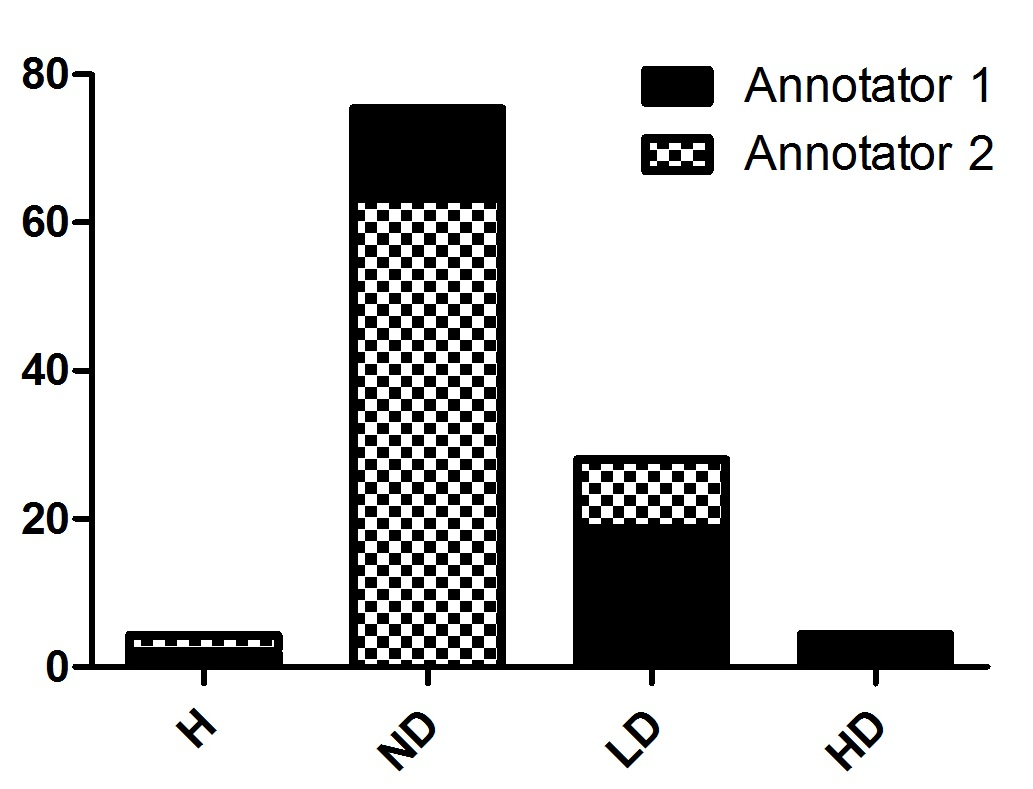
\includegraphics[scale=0.7]{ChrisCissi4cat.jpg}
\caption{Distribution of distress level annotations on the common tweets between annotators Novice 1 and Novice 2.}
\label{fig:distress-distrib1}
\end{figure}

\begin{figure}
\centering
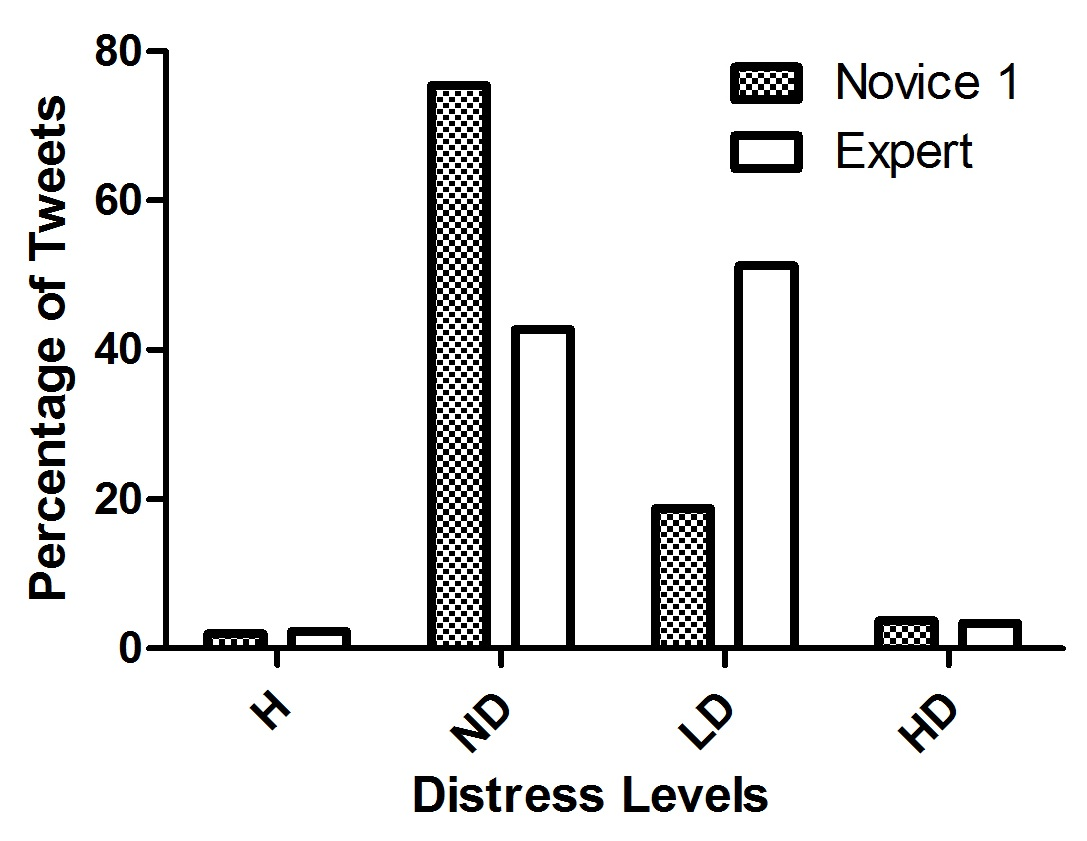
\includegraphics[scale=0.7]{ChrisMegan4Cat.jpg}
\caption{Distribution of distress level annotations from Novice 1 and Expert. Note the these two datasets are disjoint.}
\label{fig:distress-distrib2}
\end{figure}

Figures \ref{fig:distress-distrib1} and \ref{fig:distress-distrib2} show the distribution of the annotation labels each annotator makes. Interestly, the novices' distributions are fairly consistent, whereas the expert's exhibits a higher sensitivity toward distress at the high and low levels than either of the novice's.  


\begin{table}[h]
 \centering
\begin{tabular}{|c|c|}
\hline
\textbf{Group}                    & \textbf{Kappa}  \\ \hline
LIWC              & 0.3562 \\ \hline
Thematic Category & 0.5567 \\ \hline
250 Tweets               & 0.4925 \\ \hline
\end{tabular}
\caption {Inter Annotator Agreement for Novice 1 and 2}
\end{table}


\begin{table}[h]
\centering
\begin{tabular}{c|c|l|l|l|}
\cline{2-5}
                         & H                       & ND & LD & HD \\ \hline
\multicolumn{1}{|c|}{H}  & 0                       & 2  & 0  & 0  \\ \hline
\multicolumn{1}{|c|}{ND} & 1                       & 85 & 2  & 1  \\ \hline
\multicolumn{1}{|c|}{LD} & 0                       & 22 & 9  & 0  \\ \hline
\multicolumn{1}{|l}{HD}  & \multicolumn{1}{|l|}{0} & 1  & 0  & 2  \\ \hline
\end{tabular}
\caption {Confusion Matrix for LIWC for Novice 1 and 2}
\end{table}

\begin{table}[h]
\centering
\begin{tabular}{c|c|l|l|l|}
\cline{2-5}
                         & H                       & ND & LD & HD \\ \hline
\multicolumn{1}{|c|}{H}  & 4                       & 6  & 0  & 0  \\ \hline
\multicolumn{1}{|c|}{ND} & 0                       & 55 & 12 & 1  \\ \hline
\multicolumn{1}{|c|}{LD} & 0                       & 12 & 22 & 5  \\ \hline
\multicolumn{1}{|l}{HD}  & \multicolumn{1}{|l|}{0} & 1  & 0  & 4  \\ \hline
\end{tabular}
\caption {Confusion Matrix for Thematic Category for Novice 1 and 2}
\end{table}

\begin{table}[h]
\centering
\begin{tabular}{c|c|l|l|l|}
\cline{2-5}
                         & H                       & ND  & LD & HD \\ \hline
\multicolumn{1}{|c|}{H}  & 4                       & 8   & 0  & 0  \\ \hline
\multicolumn{1}{|c|}{ND} & 0                       & 150 & 14 & 2  \\ \hline
\multicolumn{1}{|c|}{LD} & 0                       & 34  & 31 & 5  \\ \hline
\multicolumn{1}{|l}{HD}  & \multicolumn{1}{|l|}{0} & 2   & 3  & 4  \\ \hline
\end{tabular}
\caption {Confusion Matrix for 250 tweets for Novice 1 and 2}
\end{table}


\begin{table}[h]
\centering
\begin{tabular}{c|c|l|}
\cline{2-3}
                         & ND  & D   \\ \hline
\multicolumn{1}{|c|}{ND} & 153 & 16  \\ \hline
\multicolumn{1}{|c|}{D}  & 36  & 150 \\ \hline
\end{tabular}
\caption {Confusion Matrix for 250 tweets for Novice 1 and 2}
\end{table}


\begin{table}[h]
\centering
\begin{tabular}{c|c|l|}
\cline{2-3}
                         & ND & D  \\ \hline
\multicolumn{1}{|c|}{ND} & 88 & 3  \\ \hline
\multicolumn{1}{|c|}{D}  & 23 & 45 \\ \hline
\end{tabular}
\caption {Confusion Matrix for LIWC tweets for Novice 1 and 2}
\end{table}

\begin{table}[h]
\centering
\begin{tabular}{c|c|l|}
\cline{2-3}
                         & ND & D  \\ \hline
\multicolumn{1}{|c|}{ND} & 65 & 13 \\ \hline
\multicolumn{1}{|c|}{D}  & 23 & 34 \\ \hline
\end{tabular}
\caption {Confusion Matrix for Thematic Category tweets for Novice 1 and 2}
\end{table}


\begin{table}[h]
\footnotesize
\begin{tabular}{|p{0.8cm}|p{4.25cm}|p{1.2cm}|}
\hline
%\textbf{64:}                         & Date: XXXX                                                                                                        & Category: suicide\_ideation \\ \hline
-3:                                  & i wish i had an older brother...                                                                                                             & {[}-0:06:08{]}              \\
-2:                                  & i'll be alright though. one day...                                                                                                           & {[}-0:02:38{]}              \\
-1:                                  & @XXXX yeah i'll be alright, it must be a phase...                                                                                          & {[}-0:02:00{]}              \\
\textgreater\textgreater\textgreater & i'm not committing suicide or anything of that nature so don't panic. maybe i'm going through a phase, maybe not. just tired of loneliness.  & \textless\textless\textless \\
1:                                   & @XXXX that's easier said then done though, you don't just break out of it overnight bro. especially if you've been a loner for a while.. & {[}+0:07:07{]}              \\
2:                                   & @silentbx i hear you.                                                                                                                        & {[}+0:07:37{]}              \\
3:                                   &   N/A                                                                                                                                           & {[}+0:07:56{]}              \\ \hline
%Msg\_id: 14481906554,                & Distress: HD                                                                                                                                 & suicide\_ideation: Y        \\ \hline
\end{tabular}
\caption{Example of a tweet labeled for high distress (HD).}
\label{fig-hdeg1}
\end{table}


\begin{table}[h]
\footnotesize
\begin{tabular}{|p{0.8cm}|p{4.25cm}|p{1.2cm}|}
\hline
%\textbf{64:}                         &Date: XXXX                                                                                                     & Category: suicide\_ideation \\ \hline
-3:                                  & highed up right now watching bloopers                                                                                                              & {[}-11:33:54{]}              \\
-2:                                  & rt @XXXX: good morning to everybody !!!!                                                                                                            & {[}-8:25:21{]}              \\
-1:                                  & hate in my heart                                                                                                        & {[}-0:38:44{]}              \\
\textgreater\textgreater\textgreater & i need to leave this world for good  & \textless\textless\textless \\
1:                                   & i need a break from life & {[}+0:00:33{]}              \\
2:                                   & all you hypocrites of the world will perish in hell one day                                                                                                                        & {[}+1:29:39{]}              \\
3:                                   & watching every body hates chris                                                                                                                                           & {[}+2:02:56{]}              \\ \hline
%Msg\_id: 14481906554,                & Distress: HD                                                                                                                                 & suicide\_ideation: Y        \\ \hline
\end{tabular}
\caption{Another example of a tweet labeled for high distress (HD).}
\label{fig-hdeg2}
\end{table}

\begin{table}[h]
\tiny
\centering
\begin{tabular}{|>{\centering\arraybackslash}m{1.2in}| >{\centering\arraybackslash}m{1.2in}|}
\hline
HD & Random \\ \hline
feel like, wanna cry, get hurt, miss 2, ima miss, win lose, tired everything, broke bitches, gun range, one person & good morning, last night, happy birthday, look like, bout 2, can't wait, video , know (cont), chris brown, jus got \\ \hline
commit suicide, miss you!, miss baby, feel empty, committing suicide, tired living, sleep forever, lost phone, left alone, :( miss & feel like, let know, make sure, bout go, time get, don't get, wats good, . ., don't want, jus saw \\ \hline
hate job, feel sad, tummy hurts, lost friend, feel helpless, leave alone, don't wanna, worst feeling, leave world, don't let & don't know, let's go, looks like, what's good, go sleep, even tho, hell yea, new single, r u?, don't wanna \\ \hline
\end{tabular}
\caption{Topic Analysis on bigrams of High Distress and Random Tweets }
\label{tab:tm}
\end{table}


\begin{table}[h]
\small
\begin{tabular}{|l|l|l|l|l|}
\hline
Train Set         & Test Set          & Precision & Recall & F-Measure \\ \hline
N1          & N1          & 0.53      & 0.63   & 0.58      \\ \hline
N1          & E & .58       & 0.27   & .37       \\ \hline
E           & E     & 0.59      & 0.71   & 0.64      \\ \hline
E            & N1          & 0.34      & 0.85   & 0.48      \\ \hline
N1 + E & N1 + E & 0.33      & 0.41   &  0.37         \\ \hline
\end{tabular}
\caption{Perform of SVN-based classification when the training and testing sets are alternately Novice 1 (N1) or the Expert (E). In cases where the training and test source coincide, the test set is a held-out set of 100 randomly selected (or 200 when N1 and E both used as in the last row) tweets. Otherwise, the training and test sets have 1000 tweets each and are disjoint.}
\end{table}

\begin{comment}
\subsection{Geography and Emotional Language}
\begin{figure}
  \centering
  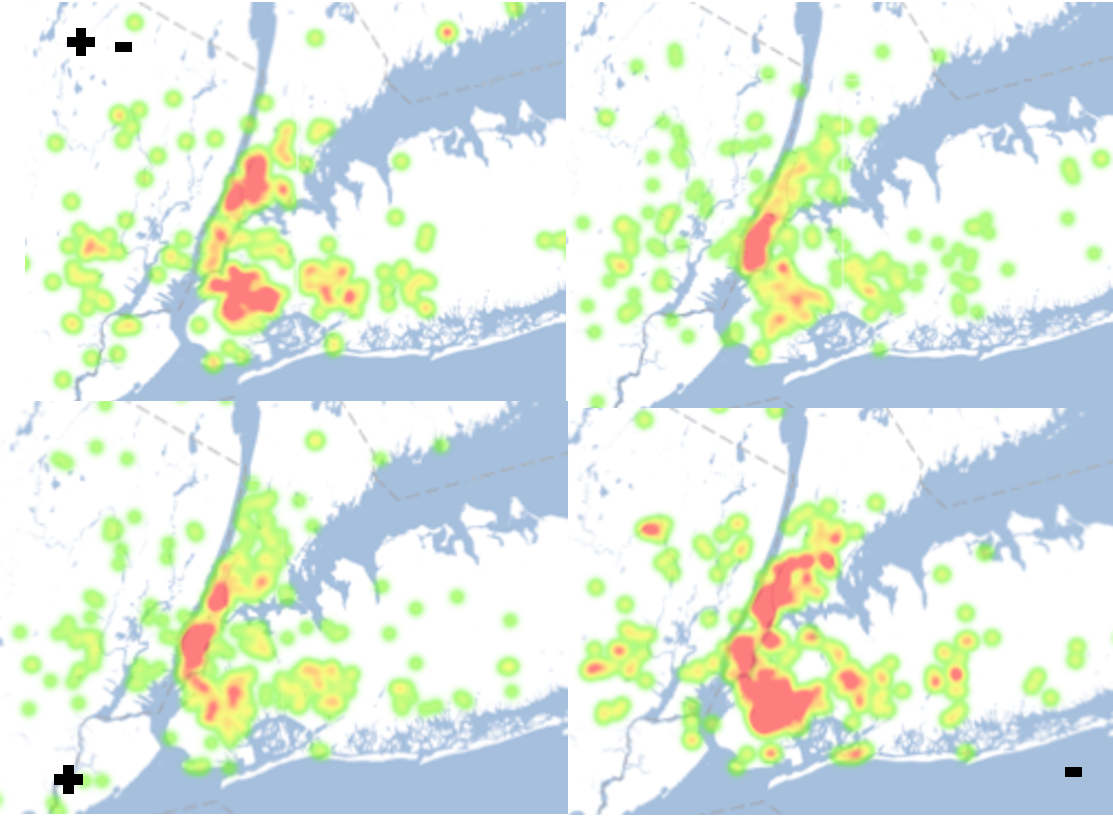
\includegraphics[scale=.4]{nyc-emo.pdf}
  \caption{Heatmaps showing the most common tweet location for those individuals who (clockwise from upper left) are among the top 25\% in using negative and positive emotional language, in the bottom 25\%  of both categories, in the top 25\% of negative language and bottom 25\% of positive language, and in the top 25\% of positive language and bottom 25\% of negative language.}
  \label{fig:geo}
\end{figure}

\subsection{Strength of Ties}
One of the fundamental properties of social networks appears to be \emph{tie strength}, or how ``close'' socially two people are. A large body of literature suggests that people are more likely to share personal information with stronger ties, and that weak ties play an important role in providing new information.  
Measuring tie strength is problematic, as there is no gold standard here. Social networking services seem to exacerbate the disparity between strong and weak ties, as many have ``friends'' or ``followers'' whom they may not even know personally, and also create their own problems and opportunities for estimating tie strength. In large-scale network analysis, researchers have sometimes characterized tie strength by the 
\emph{embeddedness} of an edge, which is the number of friends in common that two actors sharing a tie have. Highly embedded links are part of a strong social fabric, and represent strong ties. Another method of estimating tie strength is to measure the amount of activity between users. In this study, we investigate both the role that embeddness and activity play in correlating suicide-related language. 

Figure~\ref{fig:strength} shows how the use of sad language (measure by the LIWC sad feature) correlates among users sharing different tie strength and between personal and broadcast messages.

\begin{figure}
\centering
\begin{tabular}{cc}
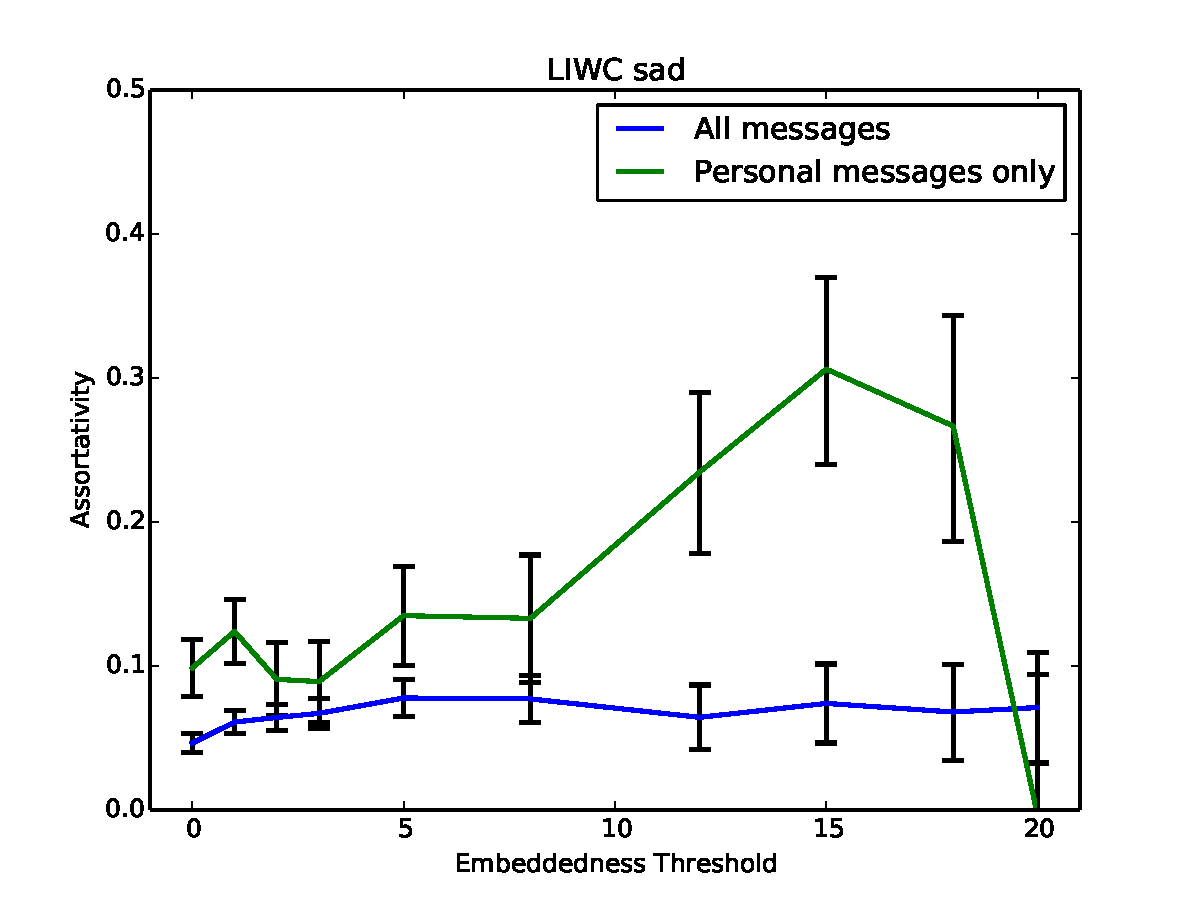
\includegraphics[scale=.2]{sad_corr.pdf} &
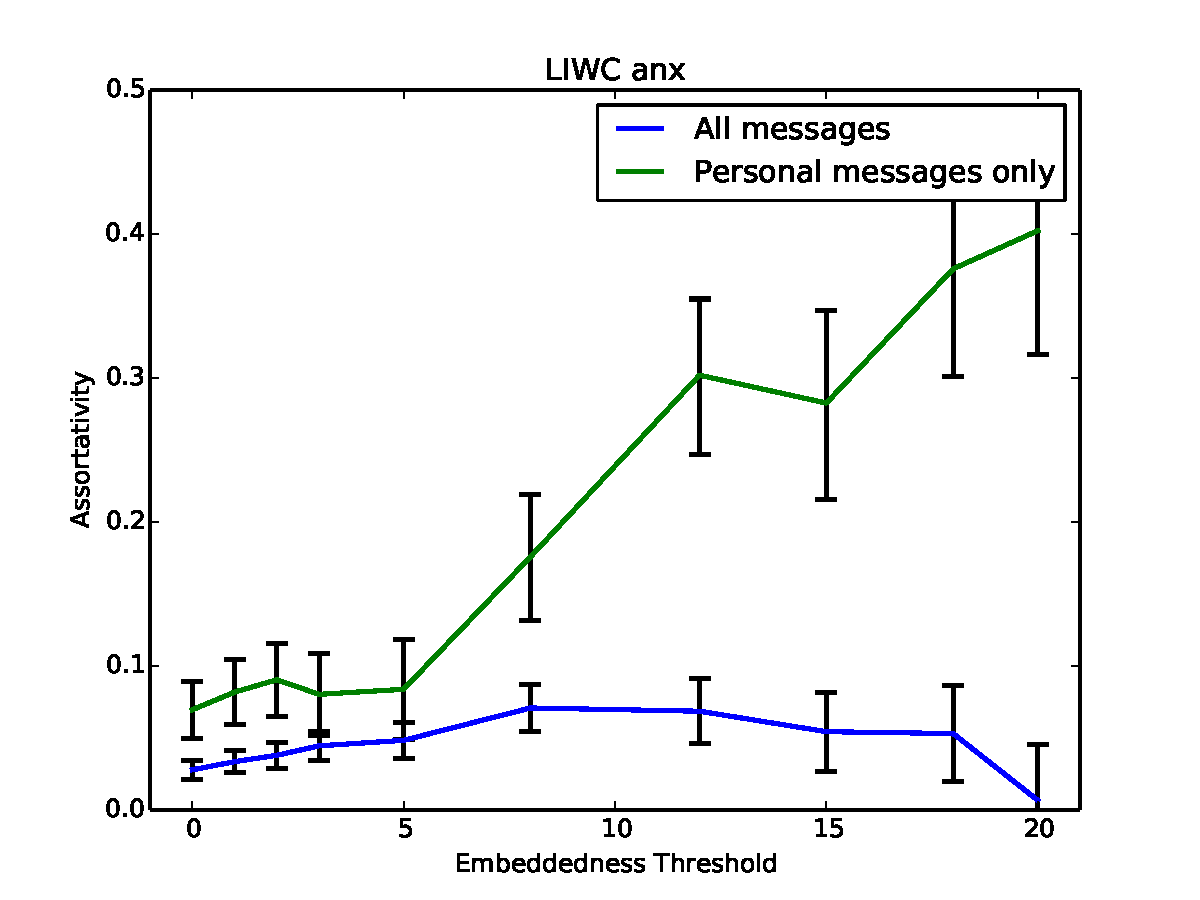
\includegraphics[scale=.2]{anx_corr.pdf} \\
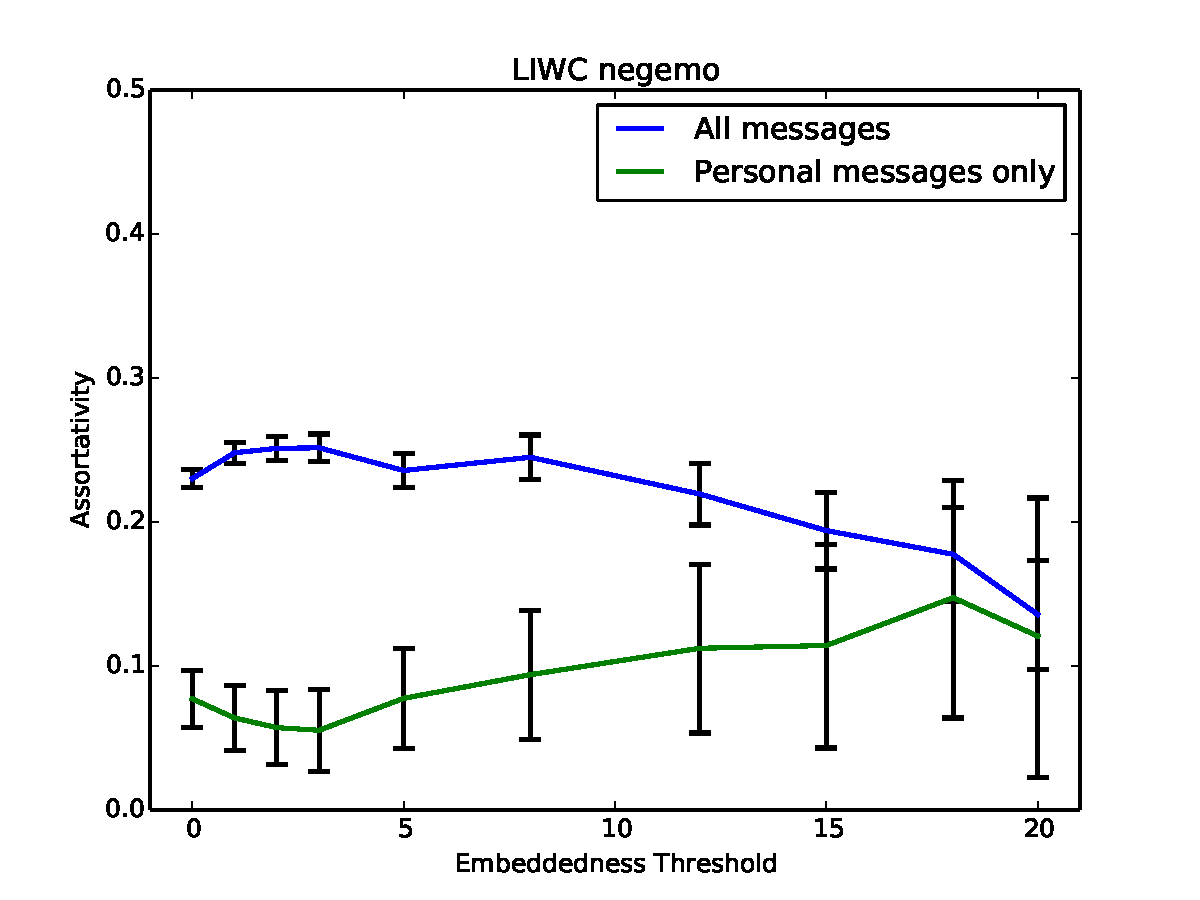
\includegraphics[scale=.2]{negemo_corr.pdf} &
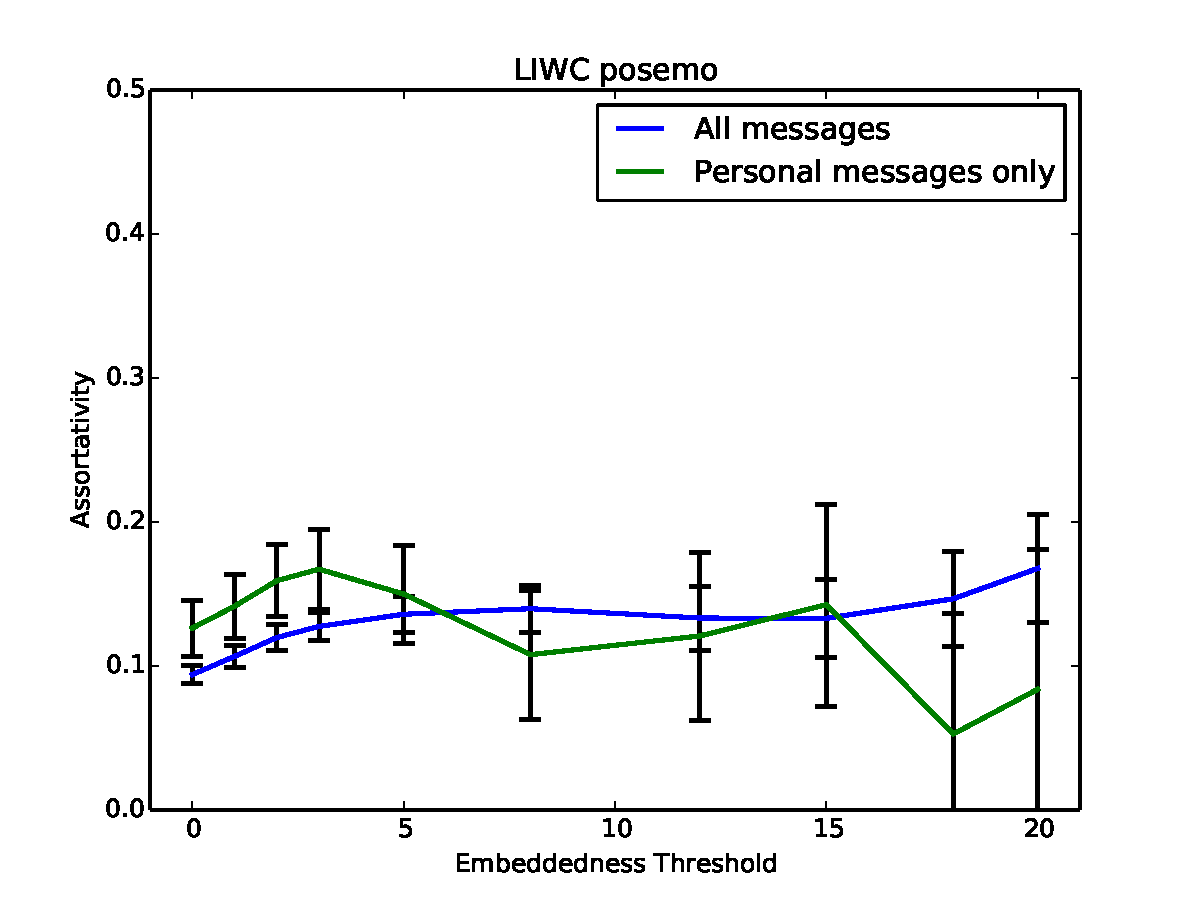
\includegraphics[scale=.2]{posemo_corr.pdf}\\
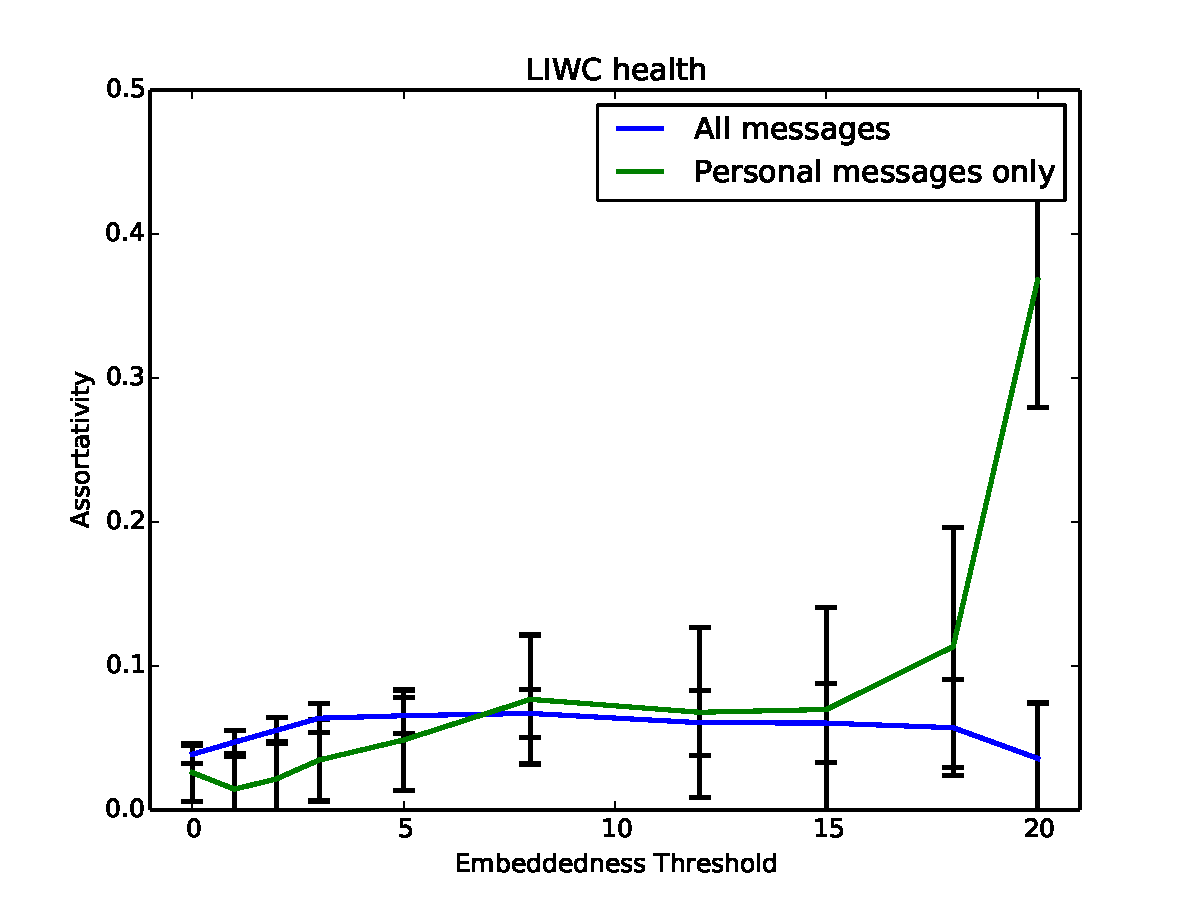
\includegraphics[scale=.2]{health_corr.pdf} &
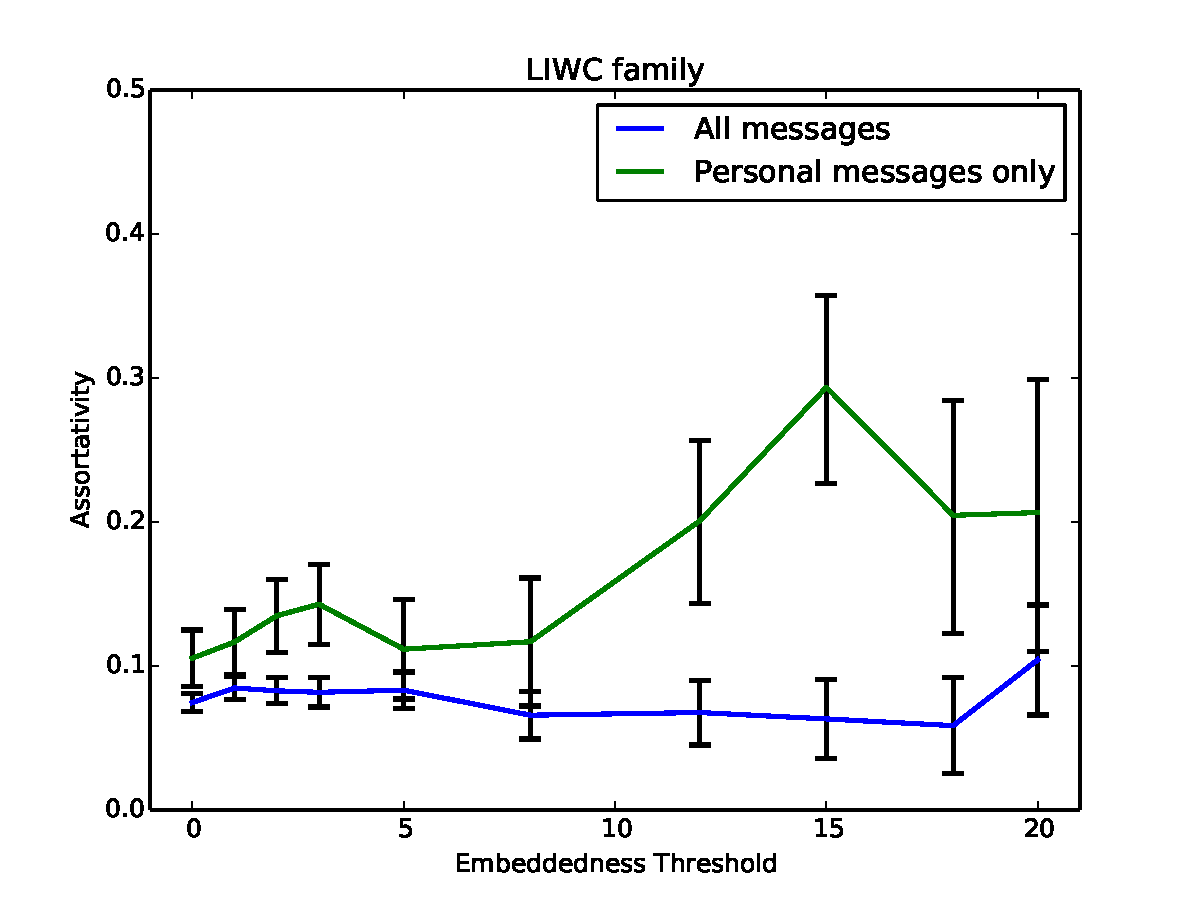
\includegraphics[scale=.2]{family_corr.pdf}
\end{tabular}
\label{fig:strength}
  \caption{Correlations between twitter friends of various LIWC scores increase as the strength of ties increase, while others behave very differently. Interestingly, two of the LIWC scores most closely associated with distress, sadness and anxiety, are among those most strongly affected by ignoring those friendships having fewer than a certain number mutal friends (i.e., embeddedness).}
\end{figure}
\end{comment}

\section{Discussion}

As previously mentioned, many of the risk factors for suicidal behavior may be linked to other expressions of distress such as aggression and interpersonal violence (Mann et al., 1999).  The goal of this study is to classify whether or not tweets were related to distress in order to determine the feasibility of classifying suicidal behaviors.  However, due to the overlap between internal and external expressions of anger, it is difficult to classify suicidal behavior without more contextual information.  Consistent with the stress diathesis model for suicidal behavior, aggression was an emerging theme that arose from the data. A number of individuals tweeted about feeling empty, hopeless, angry, frustrated, and alone.  While these are risk factors for internalizing aggression (i.e., suicidal behavior); these states are also associated with externalizing aggression.  In addition to overt expressions of anger and violence, many of the humorous tweets had an aggressive undertone. 

\begin{comment}
 Individuals often exert dominance by using pejorative and derogatory language, and the content of these tweets was often suggestive of past or current distress.  
\end{comment}



%There are unique challenges in annotating data from Twitter.  Aside from having to become familiar with different types of slang and abbreviations that could have multiple meanings, this format provides limited background context to inform the annotation process.  

Figures~\ref{fig-hdeg1}--\ref{fig-hdeg2} show examples of two tweets labeled as high distress by two annotators, along with the contextual tweets provided to help the annotation process. 
Beyond the targeted annotation categories of distress level, there were emerging themes of aggression, privilege and oppression, and daily struggles, among other.  As a result of the aggressive context, personal bias may have impacted annotation decisions. For instance, numerous tweets contained sarcasm and dark humor which may result in annotators underestimating or overlooking actual distress. In addition, by pulling data from Twitter, critical information such as pictures and the context behind information that has been retweeted was not available.  Specifically, a few individuals retweeted in a humorous manner about what individuals should say to someone who considering suicide; however, without any knowing the circumstances of the original message it was difficult to classify this tweet.  %It could represent dark humor or it could be a form of bullying.


\subsection{Limitations}
As ground truth, we rely on tweets hand-annotated by experts and non-experts. However, the mental state of another individual, observed from a line or two of text  often written in an informal register is necessarily hard to discern and, even under less noisy conditions, extremely subjective; even the observers' personal understandings of such concepts as ``distress'' may differ drastically. This makes inter-annotator agreement quite a challenge, to say nothing of observation in some objective fashion of the true mental state.


Higher levels of suicidal ideation have an inverse relationship with all types of help-seeking and a positive correlation with the decision to not seek support \cite{deane2001suicidal}. Thus we would expect suicidal individuals to generally be less active on social media than those who are not. (Fortunately, a number of studies have shown a positive correlation between online social network use and negative mood. Perhaps this means in part that individuals who are depressed are slower to disengage on- rather than off-line.)
 Part of the problem in assessing the effectiveness of self-reporting is the relative rareness by which suicide occurs, and by the inherent subjectivity of the act, which makes any data on suicide fuzzy.


\subsection{Tools Used}
 
\section{Conclusion and Future Work}
\section*{Acknowledgments}


% include your own bib file like this:

\bibliographystyle{acl}
\bibliography{acl2014-clcpws}

\begin{comment}
\begin{table*}
    \centering
    \begin{tabulary}{500pt}{|C|C|}
    \hline
    \textbf{Suicide Risk Factor Category} & \textbf{Search Terms and Phrases} \\ \hline
    Depressive Feelings & ~  me abused depressed, tired of living,so depressed,leave this world, wanna die,me hurt depressed, feel hopeless depressed, feel alone depressed, i feel helpless, i feel worthless, i feel sad, i feel empty, i feel anxious, hate my job, feeling guilty, deserve to die, desire to end own life, feeling ignored, tired of everything, feeling blue, have blues                                                                                                                                                                                                                                                                                                                                                                                                                                                                         \\ \hline
    Depression Symptoms                   & sleeping pill, sleeping a lot, i feel irritable, i feel restless, have insomnia, sleep forever,sleep disorder                                                                                                                                                                                                                                                                                                                                                                                                                                                                                                                                                                                                                                                                                                                             \\ \hline
   Drug Abuse                            & depressed alcohol, sertraline, zoloft, prozac, pills depressed, clonazepam, drug overdose, imipramine                                                                                                                                                                                                                                                                                                                                                                                                                                                                                                                                                                                                                                                                                                                                     \\ \hline
  Prior Suicide Attempts                & suicide once more, me abused suicide, pain suicide, tried suicide                                                                                                                                                                                                                                                                                                                                                                                                                                                                                                                                                                                                                                                                                                                                                                         \\ \hline
  Suicide Around Individual             & mom suicide tried, sister suicide tried, brother suicide tried, friend suicide, suicide attempted, suicide attempt                                                                                                                                                                                                                                                                                                                                                                                                                                                                                                                                                                                                                                                                                                                        \\ \hline
   Suicide Ideation                      & commit suicide,committing suicide,feeling suicidal, suicide thought about, thoughts suicide, think suicide, thought killing myself, used thought suicide, once thought suicide, past thought suicide, multiple thought suicide, want to suicide, shoot myself, a gun to head, hang myself, intention to die                                                                                                                                                                                                                                                                                                                                                                                                                                                                                                                               \\ \hline
   Self Harm                             & stop cutting myself, hurt myself, cut myself                                                                                                                                                                                                                                                                                                                                                                                                                                                                                                                                                                                                                                                                                                                                                                                              \\ \hline
   Bullying                              & i am being bullied, i have been cyber bullied, was bullied, feel bullied, stop bullying me, keeps bullying me, always getting bullied                                                                                                                                                                                                                                                                                                                                                                                                                                                                                                                                                                                                                                                                                                     \\ \hline
   Gun Ownership                         & gun suicide, shooting range went, gun range my                                                                                                                                                                                                                                                                                                                                                                                                                                                                                                                                                                                                                                                                                                                                                                                            \\ \hline
   Psychological Disorders               & diagnosed schizophrenia, diagnosed anorexia, diagnosed bulimia, i diagnosed ocd, i diagnosed bipolar, i diagnosed ptsd, diagnosed borderline personality disorder, diagnosed panic disorder, diagnosed social anxiety disorder, diagnosed post traumatic stress disorder, sleep apnea                                                                                                                                                                                                                                                                                                                                                                                                                                                                                                                                                     \\ \hline
   Family Violence Discord               & dad fight again, parents fight again, lost my friend, argument with wife, argument with husband, shouted at each other                                                                                                                                                                                                                                                                                                                                                                                                                                                                                                                                                                                                                                                                                                                    \\ \hline
   Impulsivity                           & i impulsive, i am impulsive                                                                                                                                                                                                                                                                                                                                                                                                                                                                                                                                                                                                                                                                                                                                                                                                               \\ \hline \hline
   LIWC Sad                                   & abandon, ache, aching, agoniz, agony, alone, broke,cried, cries, crushed, cry, crying, damag, defeat, depress, depriv, despair, devastat, disadvantage, disappoint, discourag, dishearten, disillusion, dissatisf, doom, dull, empt, fail, fatigu, flunk, gloom, grave, grief, griev, grim, heartbreak, heartbroke, helpless, homesick, hopeless, hurt, inadequa, inferior, isolat, lame, lone, longing, lose, loser, loses, losing, loss, lostlow, melanchol, miser, miss, missed, misses, missing, mourn, neglectoverwhelm, pathetic, pessimis, piti, pity , regret, reject, remorse, resign, ruin, sad, sadde, sadly, sadness, sob, sobbed, sobbing, sobs, solemn, sorrow, suffer, suffered, sufferer, suffering, tears, traged, tragic , unhapp,unimportant, unsuccessful, useless, weep, wept, whine, whining, woe, worthless, yearn \\ \hline

  
    \end{tabulary}
\caption{Search phrases for categories}
  \label{tab:filter}
\end{table*}
%  remember to run:
% latex bibtex latex latex
% to resolve all references
\end{comment}
\end{document}
